\chapter{Diffrazione}%Diffrazione
\section{Fenomeni di diffrazione di Fraunhofer e di Fresnel}%Fenomeni di diffrazione di Fraunhofer e di Fresnel
La \b{diffrazione} è un particolare fenomeno di interferenza che si verifica quando un'onda incontra nel suo percorso un ostacolo o un'apertura.

Un'onda arriva su uno schermo opaco nel quale è praticato un foro di dimensioni confrontabili con la lunghezza d'onda della luce incidente; uno schermo, o una pellicola fotografica riceve la luce che ha attraversato il foro.

Per il calcolo dell'ampiezza luminosa in un punto dello schermo si usa il \b{principio di Huygens-Fresnel-Kirchhoff}: \emph{ogni elemento $d\Sigma$ di una superficie d'onda $\Sigma$ si può considerare formalmente come una sorgente di onde secondarie sferiche la cui ampiezza, proporzionale all'ampiezza dell'onda primaria e all'area $d\Sigma$, varia con l'angolo secondo la funzione $f\(\theta\)$. La perturbazione prodotta in un punto $P$ si può sempre ottenere come sovrapposizione di tutte le onde sferiche elementari che raggiungono $P$.}
\begin{equation}\begin{split}
dE=\frac{Af\(\theta\)d\Sigma}{s}, \qquad f\(\theta\)=\frac{1+\cos{\theta}}{2}
\end{split}\end{equation}
L'ampiezza in $P$ si ottiene sommando vettorialmente i contributi $dE$.

\subsection{Diffrazione di Fraunhofer}
\begin{center}
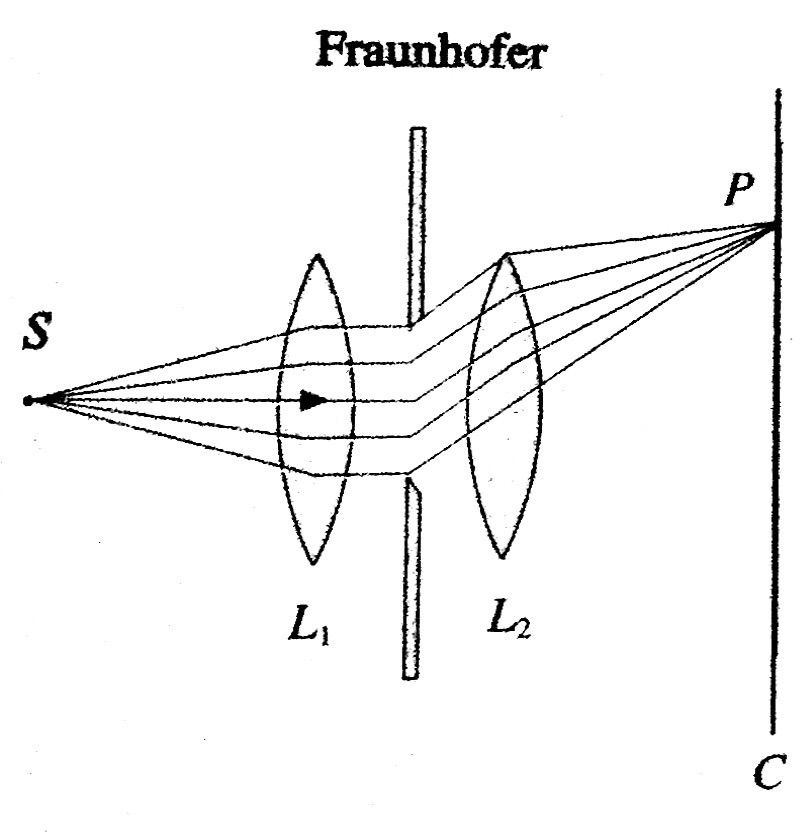
\includegraphics[width=2in]{immagini/fraunhofer.jpg}
\end{center}

La sorgente di luce e lo schermo sono a grande distanza dall'apertura. I fronti d'onda che giungono su questa sono piani e tali sono anche i fronti d'onda che giungono in $P$ provenienti dall'apertura.

Si realizza in laboratorio con due lenti: la prima trasforma l'onda sferica proveniente dalla sorgente in un'onda piana con fronte d'onda che contiene l'apertura, la seconda focalizza in un punto i raggi provenienti dall'apertura secondo una stessa direzione.

\subsection{Diffrazione di Fresnel}
\begin{center}
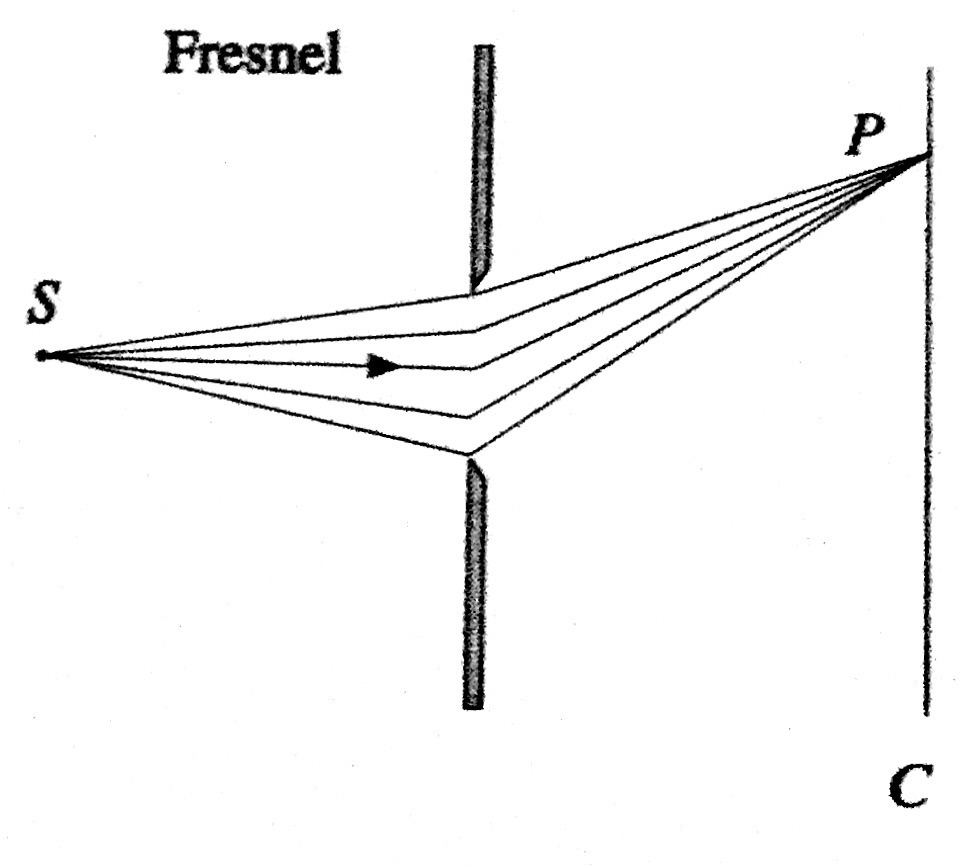
\includegraphics[width=2in]{immagini/fresnel.jpg}
\end{center}

La sorgente e lo schermo sono a distanza finita dall'apertura, i fronti d'onda non sono piani e i raggi che arrivano nel punto non sono paralleli; la stessa situazione può essere considerata per un ostacolo generico.

\section{Diffrazione ad una fenditura rettilinea}%Diffrazione ad una fenditura rettilinea
\subsection{Foro rettangolare su schermo opaco - fenditura rettilinea}
\begin{center}
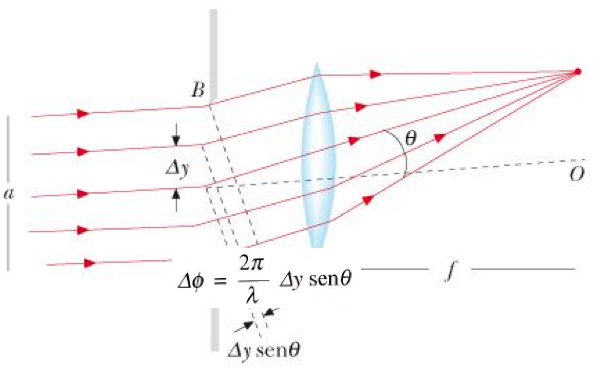
\includegraphics[width=3.5in]{immagini/huygens-fresnel.png}
\end{center}

La larghezza è $a=AB$ e la lunghezza è $L\gg a$. Sulla fenditura incide un'onda piana di lunghezza d'onda $\lambda$, con il fronte d'onda parallelo al piano contenente la fenditura (suddivisa in $N$ strisce parallele di larghezza $\Delta y$). Ciascuna striscia funge da sorgente di onde secondarie e contribuisce con l'ampiezza $\Delta E$ al campo elettrico risultante. Tutti questi contributi hanno una \b{differenza di fase}:
\begin{equation}\begin{split}
\Delta\phi=\frac{2\pi}{\lambda}\Delta y\sin{\theta}
\end{split}\end{equation}
derivante dalla \b{differenza di cammino} $\Delta y\sin{\theta}$.

Si costruisce una poligonale degli $N$ vettori rotanti che rappresentano le onde che si sovrappongono. Tendendo $N\to\infty$, $\Delta y\to 0$, la poligonale diventa un arco di circonferenza di raggio $\rho$ con \b{angolo al centro}:
\begin{equation}\begin{split}
\alpha=\frac{2\pi}{\lambda}a\sin{\theta}
\end{split}\end{equation}
uguale alla differenza di fase delle onde emesse nei punti estremi della fenditura.
\begin{center}
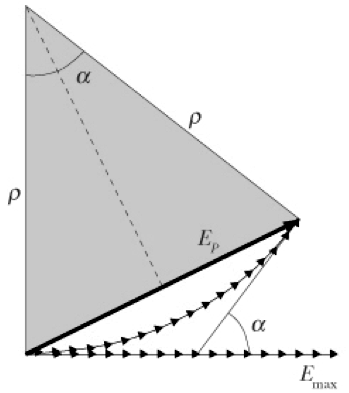
\includegraphics[width=2in]{immagini/campo-fasori.png}
\end{center}
Si vede quindi che il \b{campo risultante} è:
\begin{equation}\begin{split}
E_R=2\rho\sin{\frac{\alpha}{2}}.
\end{split}\end{equation}

La \b{lunghezza dell'arco di circonferenza} è:
\begin{equation}\begin{split}
E_{\max}=\rho\alpha
\end{split}\end{equation}
e in definitiva si ha:
\begin{equation}\begin{split}
E_R=f\(\theta\)E_{\max}\frac{\sin{\frac{\alpha}{2}}}{\frac{\alpha}{2}}.
\end{split}\end{equation}

L'\b{intensità} è proporzionale al quadrato dell'ampiezza:
\begin{equation}\begin{split}
I\(\theta\)=I_{\max}f^2\(\theta\)\[\frac{\sin{\frac{\alpha}{2}}}{\frac{\alpha}{2}}\]^2=I_{\max}f^2\(\theta\)\[\frac{\sin{\(\frac{\pi a\sin{\theta}}{\lambda}\)}}{\frac{\pi a\sin{\theta}}{\lambda}}\]^2.
\end{split}\end{equation}
\begin{center}
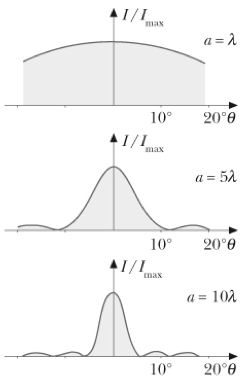
\includegraphics[width=2in]{immagini/intensitydiff1.png}
\end{center}
\begin{center}
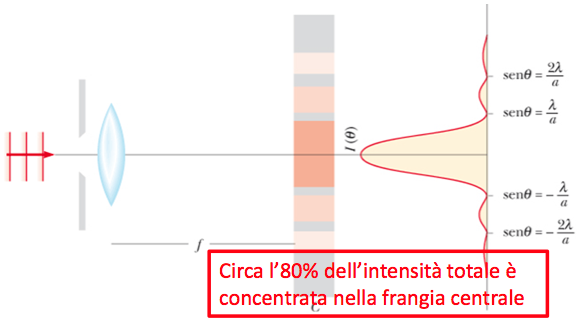
\includegraphics[width=4in]{immagini/intensitydiff2.png}
\end{center}

\subsubsection{Minimi di diffrazione}
Si hanno quando:
\begin{equation}\begin{split}
\frac{\pi a\sin{\theta}}{\lambda}=m\pi, \qquad \sin{\theta}=m\frac{\lambda}{a}, \qquad m=1,2,\dots
\end{split}\end{equation}
I primi minimi si hanno per:
\begin{equation}\begin{split}
\sin{\theta}=\pm\frac{\lambda}{a}
\end{split}\end{equation}
e si definisce la \b{larghezza angolare del massimo centrale di diffrazione} la quantità:
\begin{equation}\begin{split}
\Delta\(\sin{\theta}\)=\frac{2\lambda}{a}.
\end{split}\end{equation}

Per $a\gg\lambda$ il massimo è molto stretto e l'effetto della diffrazione è quasi trascurabile e il massimo si allarga se $a\to\lambda$. Se $a=\lambda$ il primo ed unico minimo si formerebbe a $\theta=\ang{90;;}$. Con $\alpha<\lambda$ l'intensità non si annullerebbe mai, cioè tutto lo spazio al di là della fenditura è illuminato.

\subsubsection{Massimi secondari}
Ciascun punto della fenditura emette onde sferiche $E=\frac{\e_0}{r}\sin{\(\omega t-kr\)}$. Suddividendo la fenditura in $M$ segmenti di lunghezza $\Delta y_i$. Il campo elettrico totale in $P$ è:
\begin{equation}\begin{split}
E=\sum_{i=1}^M{\frac{\e_L}{r_i}\sin{\(\omega t-kr_i\)\Delta y_i}}, \qquad \e_L=\frac{1}{D}\lim_{n\to\infty}{\e_0N}.
\end{split}\end{equation}
Per $M\to\infty$ e $r= r\(y\)$ si ha:
\begin{equation}\begin{split}
E=\e_L\int_{-\frac{D}{2}}^{\frac{D}{2}}{\frac{\sin{\(\omega t-kr\)}}{r}dy}
\end{split}\end{equation}
ed espandendo in serie $r\(y\)$ si ha $r=R-y\sin{\theta}+\frac{y^2}{2R}\cos^2{\theta}+\dots$ che per $R\gg D$ rende trascurabile il terzo termine della serie, per $y=\pm\frac{D}{2}$, (questa viene chiamata la \b{condizione di Fraunhofer}) e perciò si ha:
\begin{equation}\begin{split}
E=\frac{\e_LD}{R}\frac{\sin{\(\frac{kD}{2}\sin{\theta}\)}}{\frac{kD}{2}\sin{\theta}}.
\end{split}\end{equation}

Le loro posizioni si calcolano da $\frac{\sin^2{\beta}}{\beta^2}$, che sintetizza l'andamento dell'intensità, ponendo $\beta=\frac{kD}{2}\sin{\theta}$. Si hanno quindi quando:
\begin{equation}\begin{split}
\frac{\pi a \sin{\theta}}{\lambda}=\(2m'+1\)\frac{\pi}{2}, \qquad \sin{\theta}=\(2m'+1\)\frac{\lambda}{2a}, \qquad m'=1,2,\dots
\end{split}\end{equation}
il cui \b{campo} è:
\begin{equation}\begin{split}
E=\frac{\e_LD}{R}\(\frac{\sin{\beta}}{\beta}\)\sin{\(\omega t-kr\)}
\end{split}\end{equation}
e la cui \b{intensità} risulta (trascurando il fattore di inclinazione):
\begin{equation}\begin{split}
I\(\theta\)=\frac{1}{2}\(\frac{\e_LD}{R}\)^2\(\frac{\sin{\beta}}{\beta}\)^2\\
\frac{I_{m'}}{I_{\max}}=\frac{1}{\[\(2m'+1\)\frac{\pi}{2}\]^2}\simeq\frac{0.4}{\(2m'+1\)^2}
\end{split}\end{equation}

\section{Diffrazione ad un foro circolare e da parte di un disco opaco}%Diffrazione ad un foro circolare e da parte di un disco opaco
\subsection{Apertura circolare}
La figura di diffrazione consta in un disco luminoso centrale circondato da una serie di corone circolari alternativamente chiare e scure.

L'\b{angolo a cui cade il primo minimo d'intensità} è:
\begin{equation}\begin{split}
\sin{\theta}=1.22\frac{\lambda}{D}=0.61\frac{\lambda}{R}
\end{split}\end{equation}
dove $R$ è il raggio e $D$ il diametro dell'apertura. Il termine $1.22$ deriva dal calcolo eseguito secondo il principio di Huygens-Fresnel-Kirchhoff, che integra su tutte le sorgenti secondarie infinitesime anulari in cui viene suddiviso il foro.

Spesso $\lambda\ll D$ e perciò:
\begin{equation}\begin{split}
\theta=1.22\frac{\lambda}{D}=0.61\frac{\lambda}{R}
\end{split}\end{equation}
con $2\theta$ la \b{larghezza angolare dl massimo centrale}.

\subsection{Diffrazione da parte di un disco opaco}
Considerando un'onda piana monocromatica che incide su un'apertura circolare $G$ di diametro $h\gg\lambda$ e \b{ponendo sull'apertura $G$ un disco opaco $A$ di diametro $h$ avente al centro un foro circolare di diametro $D$}, in un punto $P$ dello schermo, sotto l'angolo $\theta$, si osserva un campo elettrico di ampiezza $E_A\(\theta\)$ e un'intensità $I_A\(\theta\)$ proporzionale a $E_A^2\(\theta\)$. Se invece si \b{pone al posto di $A$ un disco opaco $B$ di diametro $D$} si osserva un campo elettrico di ampiezza $E_B\(\theta\)$ e un'intensità $I_B\(\theta\)$ proporzionale a $E_B^2\(\theta\)$.

\b{Le aperture costituite dal foro nel disco $A$ e dell'anello dovuto alla presenza del disco $B$ sono complementari}. Se si sovrappongo si ha un campo $E_G\(\theta\)=E_A\(\theta\)+E_B\(\theta\)$, ed essendo $E_G\(\theta\)=0$ per $\theta\neq 0$ si ha il \b{principio di Babinet}:
\begin{equation}\begin{split}
E_B\(\theta\)=-E_A\(\theta\), \qquad I_B\(\theta\)=I_A\(\theta\)
\end{split}\end{equation}
che stabilisce che \b{con l'esclusione della direzione $\theta=0$, la figura di diffrazione prodotta da un disco opaco di diametro $D$ coincide con la figura di diffrazione prodotta da un foro circolare di diametro $D$ praticato in uno schermo opaco}.

\section{Limite di risoluzione delle lenti}%Limite di risoluzione delle lenti
Il fatto che l'immagine di un punto data da una lente sia un dischetto è importante quando si vogliono distinguere due oggetti puntiformi.

\subsubsection{Criterio di Rayleight}
Quando due sorgenti sono viste da una lente sotto un angolo:
\begin{equation}\begin{split}
\alpha_R=1.22\frac{\lambda}{D}
\end{split}\end{equation}
il primo minimo della figura di diffrazione di una sorgente coincide con il centro del massimo dell'altra sorgente e si dice che \b{le due sorgenti sono appena risolte}. Definendo $\alpha$ come \b{angolo minimo risolvibile} e il suo inverso come \b{potere risolutivo} o \b{separatore della lente}:
\begin{equation}\begin{split}
\rho=\frac{1}{\alpha_R}=\frac{D}{1.22\lambda}
\end{split}\end{equation}
il quale non dipende dalla distanza focale della lente, ma soltanto dalla sua apertura, e migliora al crescere di questa.

Se $\alpha\gg\theta=1.22\frac{\lambda}{D}$ non c'è sovrapposizione tra i due dischetti che rappresentano le immagini delle due sorgenti. Al diminuire di $\alpha$ le due immagini cominciano a sovrapporsi.

\subsection{Potere separatore di un telescopio}
La formula del potere risolutivo è valida anche quando il fascio luminoso, invece di essere rifratto da una lente, è riflesso da uno specchio sferico di apertura $D$ e focale $f$. Dipendendo $\alpha_R$ e $\rho$ dalla lunghezza d'onda, si ha che le prestazioni sono migliori con la luce violetta e peggiori con la luce rossa.

\subsection{Potere separatore di un microscopio}
Invece della separazione angolare è più conveniente specificare la distanza minima $s$ tra due punti distinguibili. Se \b{i due punti sono nel piano focale anteriore dell'obiettivo} essi \b{sono visti sotto l'angolo $\theta=\frac{s}{f}$}. Si definisce l'\b{angolo di accettanza $\phi$} secondo la relazione $\sin{\phi}=\frac{R}{f}$ e quindi si ottiene:
\begin{equation}\begin{split}
s=f\alpha_R=1.22\lambda\frac{f}{D}=\frac{0.61\lambda}{\sin{\phi}}=\frac{0.61\lambda_0}{n\sin{\phi}}=\frac{0.61\lambda_0}{A_n}
\end{split}\end{equation}
chiamando $n\sin{\phi}$ \b{apertura numerica $A_n$}.

\subsection{Potere separatore dell'occhio umano}
Il diametro della pupilla dell'occhio umano varia all'incirca tra i limiti $D=\SI{8}{mm}$ (caso più favorevole) e $D=\SI{2}{mm}$ (caso meno favorevole); con luce di lunghezza d'onda $\lambda_0=\SI{0.55e-6}{m}$ si ha:
\begin{equation}\begin{split}
\SI{0.84e-4}{rad}\le\alpha_R\le\SI{3.36e-4}{rad}.
\end{split}\end{equation}

\begin{center}
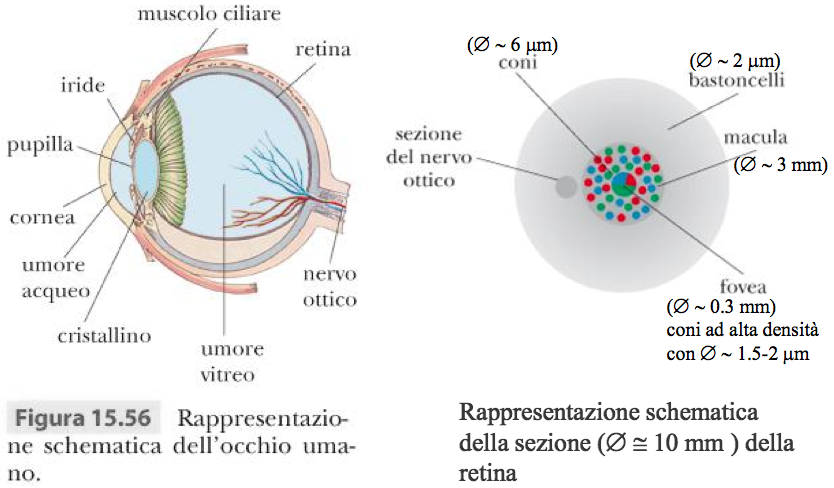
\includegraphics[width=\textwidth]{immagini/occhio.png}
\end{center}

Nel caso meno favorevole la distanza minima tra due punti ancora distinguibili dall'occhio, posti alla distanza $L=\SI{25}{cm}$ viene detta \b{visione distinta} ed è:
\begin{equation}\begin{split}
s=L\alpha_R=\SI{250}{mm}\cdot\SI{3.36e-4}{rad}=\SI{84}{\um}
\end{split}\end{equation}
che diventa $s=\SI{21}{\um}$ per il caso più favorevole con $D=\SI{8}{mm}$.

Sperimentalmente il potere separatore angolare dell'occhio è vicino a \SI{4e-4}{rad} e la distanza $s=\SI{100}{\um}$. Questo fatto dipende dalla struttura granulare della retina, posta nella parte posteriore dell'occhio.

L'occhio è formato da:
\begin{itemize}
\item \b{Fotorecettori}: cellule fotosensibili, stimolate dalla luce trasmettono un impulso di tensione (di qualche \SI{}{\uV}) alle cellule elaboratrici. Esistono due tipi di \b{fotorecettori}, che contengono sostanze fotosensibili (fotopigmenti):
\begin{itemize}
\item \b{Bastoncelli}, funzionanti nella penombra (visione scotoscopica), contengono un solo tipo di fotopigmento, la rodopsina. Qualunque sia $\lambda$, i fotoni producono la stessa eccitazione nei bastoncelli e perciò al cervello arrivano impulsi formati tutti uguali, in numero proporzionale ai fotoni assorbiti. \'E quindi impossibile discriminare i colori (tonalità del grigio). Però la sensibilità è più elevata: al buio è possibile rivelare un lampo di luce che eccita anche solo una decina di bastoncelli.
\item \b{Coni}, funzionanti in piena luce (visione fotoscopica), esistono in 3 tipi diversi, corrispondenti a 3 diversi fotopigmenti (iodopsine) che hanno un massimo di assorbimento rispettivamente nel rosso, nel verde, nel blu. L'eccitazione contemporanea dei 3 fotopigmenti con lo stesso numero di fotoni provoca la sensazione del bianco. Gli altri colori vengono percepiti per sovrapposizione di diversi numeri di impulsi formati (tutti uguali) provenienti dai 3 fotopigmenti. I daltonici mancano di un tipo (o raramente di due) di iodopsina sensazione distorta dei colori.\end{itemize}
\item \b{Cellule bipolari}: cellule che elaborano gli impulsi elettrici, dando a tutti altezza e lunghezza standard.
\item \b{Cellule gangliari}: ricevono gli impulsi formati e attraverso le fibre del nervo ottico ($\sim\SI{e7}{}$ neuroni) li trasmettono alla sezione occipitale del cervello, detta corteccia visiva (collegamento 1 a 1 con coni e 100 a 1 con bastoncelli).
\end{itemize}
\begin{center}
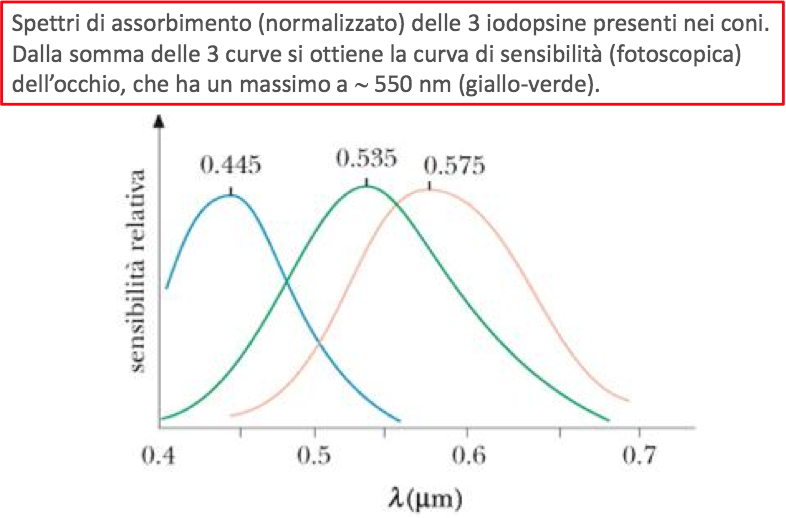
\includegraphics[width=\textwidth]{immagini/assorbimentoiodopsine.png}
\end{center}
\begin{center}
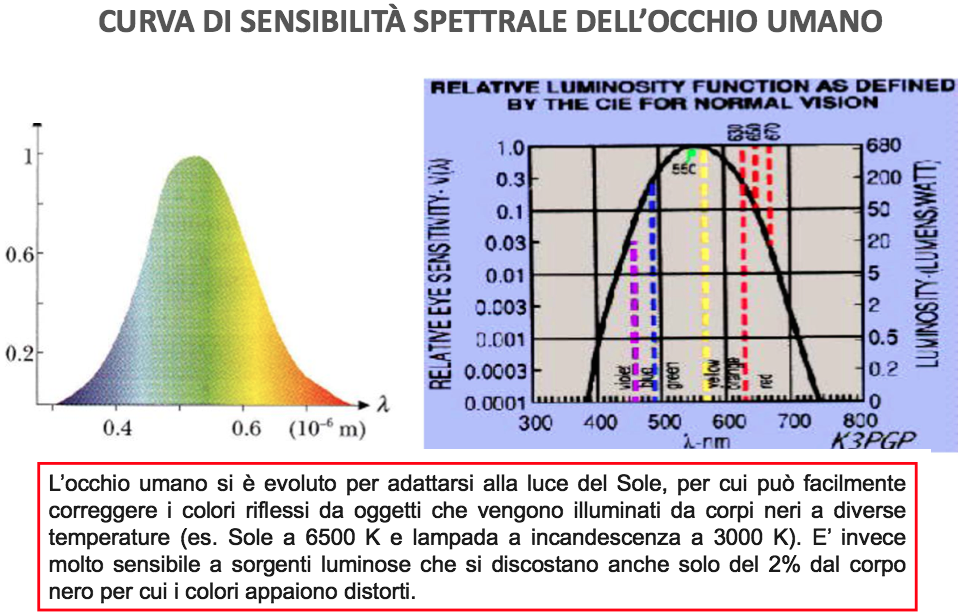
\includegraphics[width=\textwidth]{immagini/curvasensibilityocchio.png}
\end{center}

\section{Reticolo di diffrazione}%Reticolo di diffrazione
Si dispongono in modo regolare $N$ fenditure rettilinee, ciascuna di larghezza $a$, equispaziate di una distanza $d$, e si realizza un sistema di $N$ sorgenti che viene chiamato \b{reticolo di diffrazione in trasmissione}.

Un'onda piana di lunghezza d'onda $\lambda$ incide su un reticolo, che sta in un piano d'onda (l'incidenza è normale); dopo il reticolo si pone una lente convergente e si osserva la figura di intereferenza nel piano focale della lente. L'\b{intensità della singola fenditura} è:
\begin{equation}\begin{split}
I_1\(\theta\)=I_0\[\frac{\sin{\(\frac{\pi a\sin{\theta}}{\lambda}\)}}{\frac{\pi a\sin{\theta}}{\lambda}}\]^2
\end{split}\end{equation}
e quindi l'\b{intensità} in un punto è:
\begin{equation}\begin{split}
I\(\theta\)=I_0\[\frac{\sin{\(\frac{\pi a\sin{\theta}}{\lambda}\)}}{\frac{\pi a\sin{\theta}}{\lambda}}\]^2\[\frac{\sin{\(\frac{N\pi d\sin{\theta}}{\lambda}\)}}{\sin{\(\frac{\pi d\sin{\theta}}{\lambda}\)}}\]^2
\end{split}\end{equation}
e si nota che \b{l'intensità della figura di interferenza è modulata dalla diffrazione}.

\subsubsection{Massimi principali}
Si hanno lungo:
\begin{equation}\begin{split}
\sin{\theta_m}=m\frac{\lambda}{d}, \qquad m=0,\pm1,\pm2,\dots
\end{split}\end{equation}

\subsubsection{Larghezza angolare del massimo}
La distanza angolare tra un massimo principale e il minimo ad esso adiacente:
\begin{equation}\begin{split}
\Delta\(\sin{\theta}\)=\cos{\theta}\Delta\theta=\frac{\lambda}{Nd}=\frac{\lambda}{L}.
\end{split}\end{equation}
La larghezza angolare è perciò:
\begin{equation}\begin{split}
\Delta\theta_m=2\Delta\theta=\frac{2\lambda}{L\cos{\theta_m}}=\frac{2\lambda}{Nd\cos{\theta_m}}
\end{split}\end{equation}
e quindi \b{maggiore è il numero di fenditure del reticolo, più strette sono le frange prodotte}.

\subsubsection{Intensità dei massimi principali}
Quella della frangia centrale aumenta proporzionalmente a $N^2$, quella degli altri massimi invece è ridotta a causa della diffrazione:
\begin{equation}\begin{split}
\frac{I_{\max}\(m\)}{I_{\max}\(m=0\)}=R_m=\[\frac{\sin{\(m\pi\frac{a}{d}\)}}{m\pi\frac{a}{d}}\]^2.
\end{split}\end{equation}
Il rapporto dipende dal rapporto tra la larghezza delle fenditure e la loro distanza. Quando un minimo di diffrazione coincide con un massimo di interferenza, il rapporto $\frac{a}{d}=\frac{m_a}{m}$ e $R_m=0$.

\section{Potere dispersivo e potere risolutivo di un reticolo di diffrazione}%Potere dispersivo e potere risolutivo di un reticolo di diffrazione
Se la luce che illumina il reticolo non è monocromatica, le differenti lunghezze d'onda che compongono la luce incidente producono massimi principali ad angoli diversi. Solo il massimo di ordine 0 si forma a $\theta=0$. Questo fenomeno si chiama \b{dispersione angolare}.

Fissato un valore dell'ordine $m$, l'insieme dei massimi che si formano per le diverse lunghezze d'onda prende il nome di \b{spettro di ordine $m$}. Quando l'illuminazione è in luce bianca lo spettro di prim'ordine è l'unico cosiddetto \b{spettro puro}.

La dispersione e il potere risolutivo si differiscono a proprietà diverse: un reticolo con passo piccolo ha un buona dispersione, ma se è piccolo anche il numero di fenditure (al limite $N=2$) esso non è adatto a separare lunghezze d'onda molto vicine: i centri dei massimi sono ben distanziati, ma i massimi stessi sono larghi. Invece in un reticolo con passo maggiore, ma con un gran numero di fenditure, ha dispersione minore e potere risolutivo superiore, essendo i massimi molto stretti.

\subsection{Potere dispersivo di un reticolo}
Date due onde monocromatiche le cui lunghezze d'onda differiscono di $d\lambda$, i due massimi principali dello stesso ordine si formano ad angoli che differiscono di $d\theta$. Il \b{potere dispersivo} viene definito quindi:
\begin{equation}\begin{split}
D=\frac{d\theta}{d\lambda}=\frac{1}{d}\frac{m}{\cos{\theta_m}}.
\end{split}\end{equation}
\b{La dispersione aumenta al diminuire del passo del reticolo e, per un dato reticolo, all'aumentare dell'ordine dello spettro}.

\subsection{Potere risolutivo di un reticolo}
Per distinguere onde luminose con lunghezze d'onda molto vicine i massimi principali relativi a queste lunghezze d'onda devono avere larghezza angolare più piccola possibile. Il \b{potere risolutivo} del reticolo all'ordine $m$ viene definito come:
\begin{equation}\begin{split}
R=\frac{\lambda}{\Delta \lambda}=mN.
\end{split}\end{equation}
\b{Il potere risolutivo risulta proporzionale al numero totale di fenditure e aumenta con l'ordine dello spettro,} ma non dipende dal passo del reticolo.

\section{Fenomeni di diffrazione di Fresnel}%Fenomeni di diffrazione di Fresnel
Si considera un fronte d'onda piano che si propaga verso un punto $P$ e si indica con $r_0$ la distanza di $P$ dal fronte d'onda. Suddividendo questo in tante zone anulari concentriche aventi $O$ come centro, definite dalla condizione che le distanze da $P$ del bordo interno e del bordo eterno di ciascuna zona differiscano di $\frac{\lambda}{2}$. 

Il bordo del disco centrale viene chiamato \b{prima zona di Fresnel} (dista da $P$ $r_1=r_0+\frac{\lambda}{2}$) e il bordo esterno del primo anello \b{seconda zona di Fresnel}. In generale si ha:
\begin{equation}\begin{split}
r_n=r_{n-1}+\frac{\lambda}{2}=r_0+n\frac{\lambda}{2}, \qquad n=1,2,\dots
\end{split}\end{equation}

I \b{raggi delle circonferenze che limitano le zone di Fresnel} valgono:
\begin{equation}\begin{split}
R_n^2=r_n^2-r_0^2=\(r_0+n\frac{\lambda}{2}\)^2-r_0^2=nr_0\lambda+n^2\frac{\lambda^2}{4}\simeq nr_0\lambda.
\end{split}\end{equation}

Il campo elettrico in $P$ si ottiene come somma dei campi elettrici $E_n$ provenienti dalle singole zone. Le \b{aree delle zone di Fresnel} risultano tutte uguali tra loro e non dipendo da $n$:
\begin{equation}\begin{split}
\Sigma_n=\pi\(R_n^2-R_{n-1}^2\)=\pi\[nr_0\lambda-\(n-1\)r_0\lambda\]=\pi r_0\lambda.
\end{split}\end{equation}
Le \b{ampiezze delle onde emesse} dalle varie zone \b{sono diverse in $P$ soltanto a causa del fattore di inclinazione e della distanza}, diminuendo al crescere dell'ordine $n$ della zona.

La \b{differenza di fase} tra le onde emesse dai bordi interno ed esterno in ciascuna zona è:
\begin{equation}\begin{split}
\delta=\frac{2\pi}{\lambda}\(r_n-r_{n-1}\)=\frac{2\pi}{\lambda}\frac{\lambda}{2}=\pi.
\end{split}\end{equation}
Disegnando gli infiniti vettori infinitesi relativi alla prima zona di Fresnel si ottiene una semicirconferenza il cui diametro dà il campo elettrico $E_1$ dell'onda emessa dalla prima zona.

L'\b{intensità luminosa} in $P$ prodotta da un fronte d'onda indefinito \b{è pari ad un quarto dell'intensità prodotta dalla prima zona}: la diminuzione è dovuta all'interferenza distruttiva tra le varie zone.

\subsection{Diffrazione di un foro circolare}
Fissato un punto distante $r_0$ dal piano d'onda, ad ogni disco di raggio $R$ tracciato sul piano è associato, sulla curva a spirale dei vettori rotanti un punto $O''$ (ovvero un vettore la cui ampiezza dà l'ampiezza del campo elettrico $E_P$ prodotto in $P$ dalla porzione del fronte d'onda coincidente col disco). Quando $R$ uguaglia il raggio di una delle zone di Fresnel il punto $O''$ sta sulla verticale passante per $O$.

Se si interpone sul fronte d'onda uno schermo opaco con un foro di raggio $R$, si ha che $OO''$ dà l'ampiezza del campo elettrico trasmesso dal faro e l'intensità è proporzionale a $\(OO''\)^2$. I punti di \b{massima intensità} si hanno quando il foro comprende esattamente un numero dispari di zone di Fresnel, i punti di \b{minima intensità} si hanno quando il foro ricopre esattamente un numero pari di zone di Fresnel.

Se ci si pone invece che sull'asse in un punto $Q$ che non sta sull'asse, occorre tener presente che \b{il sistema di zone di Fresnel è caratteristico del punto di osservazione}.

Cambiando invece $r_0$ si cambia il sistema d'azione di Fresnel: ci sono valori di $r_0$ per i quali nel foro cadono un numero dispari di zone e valori per i quali invece le zone coincidenti col foro sono in numero pari.

\subsection{Reticolo zonato di Soret}
Nel punto $P$ si può avere un'intensità notevole se si interpone sul fronte d'onda, a distanza $r_0$, una sottile lastra di vetro in cui sono tracciate una serie di corone circolari opache disposte in modo da intercettare, per quel valore di $r_0$ e $\lambda$, le zone dispari di Fresnel lasciando scoperte quelle di ordine pari, o viceversa. Questo dispositivo viene chiamato \b{reticolo zonato di Soret}.

Se si fissano la lunghezza d'onda e le dimensioni del dischetto centrale, sono automaticamente fissati tutti i raggi delle zone di Fresnel dalla condizione che le aree delle corone circolai siano uguali ed è fissata la distanza $r_0$ che corrisponde a questo sistema di zone.

Un'onda piana monocromatica viene in parte concentrata nel punto $P$ distante $r_0$ dal centro e quindi si può considerare che si comporti come una lente convergente di focale:
\begin{equation}\begin{split}
f=r_0=\frac{R_1^2}{\lambda}=\frac{R_n^2}{n\lambda}.
\end{split}\end{equation}

\subsection{Diffrazione di un disco opaco}
Considerando la diffrazione subita da un'onda piana di lunghezza d'onda $\lambda$ incidente ortogonalmente su un disco opaco di raggio $R$ e osservando cosa succede in un punto $P$ posto a distanza $r_0$ dal disco si nota che il campo elettrico dell'onda diffratta si ottiene utilizzando il principio di sovrapposizione:
\begin{equation}\begin{split}
\E=\E_{\textrm{disco}}+\E_{\textrm{foro}}\\
\Longrightarrow \E_{\textrm{disco}}=\E-\E_{\textrm{foro}}
\end{split}\end{equation}

All'aumentare del raggio $R$, $O''\to O'$ e l'intensità tende a 0 senza mai raggiungerlo. In $P$, indipendentemente dal raggio del disco, si osserva sempre un punto chiamato \b{punto luminoso di Poisson}.

\subsection{Diffrazione di un ostacolo piano}
Considerando un ostacolo piano delimitato da uno spigolo netto e un'onda incidente piana e monocromatica, con fronte d'onda parallelo al piano contenente l'ostacolo si ottiene che se $E$ è l'ampiezza del campo elettrico prodotto in $P$ dall'intero fronte d'onda, l'ampiezza in presenza dell'ostacolo è $E_P=\frac{E}{2}$ e l'intensità è $I_P=\frac{I}{4}$.

In un punto $P_1$ distante da $P$, $R_1=\sqrt{r_0\lambda}$, la prima zona di Fresnel contribuisce completamente all'intensità; per le altre si può dire che ciascuna zona pari è tagliata un po' meno delle successiva zona dispari, così che il contributo da sottrarre è minore che in assenza dell'ostacolo e l'intensità in $P_1$ risulta maggiore dell'intensità senza ostacolo.

\section{Olografia}%Olografia
Un'onda piana monocromatica che si propaga lungo l'asse $x$ e incide su una lastra fotografica produce su questo un annerimento che dipende localmente dall'intensità che ha colpito la lastra durante il tempo di esposizione e che quindi, per l'onda piana, è uniforme.

Si suppone che in un punto $P$, posto a distanza $x_0$ dalla lastra, ci sia una sferetta molto piccola, la quale diffonde, attraverso un meccanismo, la luce incidente dando origine ad un'onda sferica coerente con l'onda primaria e quindi capace di interferire con essa. In un punto $Q$ della lastra distante $r$ da $P$ e $z$ dall'asse $x$ si osserva l'interferenza tra l'onda primaria (\b{onda riferimento}):
\begin{equation}\begin{split}
E_{\textrm{rif}}=E_0\cos{\(kx_0-\omega t\)}
\end{split}\end{equation}
e l'onda sferica proveniente da $P$ (\b{onda oggetto}):
\begin{equation}\begin{split}
E_{\textrm{ogg}}=E\(r\)\cos{\(kr-\omega t\)}.
\end{split}\end{equation}

\b{Nella figura di interferenza sono registrate le informazioni sull'ampiezza e sulla fase dell'onda diffusa che ha contribuito ad impressionare la lastra}: l'informazione sull'ampiezza è data dal grado di annerimento e quella sulla fase è contenuta nella coordinata $z$, legata a $\delta$.

Supponendo di illuminare la lastra fotografica sviluppata con lo stesso fascio di luce con cui la si è prodotta, si ha che la struttura degli anelli chiari e scuri che costituiscono l'ologramma è caratteristica di un reticolo zonato di Soret; il raggio del dischetto scuro centrale, uguale al raggio della prima posizione di minimo, vale $z_1=\sqrt{x_0\lambda}$ ed è uguale al raggio della prima zona di Fresnel relativa ad un punto $P'$ distante $x_0$ dall'ologramma. Le onde diffratte dalle aperture anulari (anelli chiari) vengono focalizzate nel punto distante
\begin{equation}\begin{split}
f=\frac{z_1^2}{\lambda}=x_0.
\end{split}\end{equation}

Si dice che $P'$, simmetrico del punto $P$, è l'\b{immagine reale} dell'oggetto puntiforme $P$. I raggi diffratti sembrano provenire dalla posizione in cui era stato posto l'oggetto $P$ e per questa ragione si dice che l'ologramma fornisce anche un'\b{immagine virtuale} dell'oggetto, situata nella stessa posizione e completamente indistinguibile da questo. I raggi che sembrano provenire da $P$ soddisfano alle stesse condizioni di coerenza valide per i raggi che convergono in $P'$ e portati ad interferire sulla retina danno anch'essi un massimo.

Se invece di un oggetto puntiforme nell'introno di $P$ è posto un oggetto vero e proprio trasparente, ciascun elemento dà origine alla sua figura di interferenza e quindi al suo reticolo di Soret e l'ologramma è la sovrapposizione di un numero grandissimo di reticoli. L'immagine reale, che ha le stesse proprietà rispetto all'oggetto dell'immagine data da uno specchio piano, può essere osservata mettendola a fuoco su uno schermo. L'immagine virtuale è visibile ad occhio nudo guardando attraverso l'ologramma. Si tratta di \b{immagini veramente tridimensionali}.

L'originalità della procedura olografica consiste nella registrazione dell'informazione completa relativa al fronte d'onda emesso dall'oggetto e successivamente nella possibilità di ricostruire questo fronte d'onda come se fosse emesso dall'oggetto stesso.

\section{Diffrazione dei raggi $X$}%Diffrazione dei raggi $X$
In un normale reticolo di diffrazione ottico i raggi $X$ non vengono praticamente diffratti; un reticolo spaziale naturale adatto a produrre la diffrazione dei raggi $X$ è un reticolo cristallino, in cui gli atomi sono disposti secondo strutture regolare con distanze reciproche molto piccole.

In un cristallo di \ce{Na^+Cl^-} si forma un reticolo cubico di lato $a$ chiamata \b{costante reticolare} (che nel caso specifico vale \SI{0.282}{nm}). Quando un fascio di raggi $X$ di lunghezza d'onda $\lambda$ incide su questa struttura di atomi, gli elettroni che circondano ogni singolo nucleo si comportano come dipoli oscillanti, emettendo radiazione elettromagnetica di lunghezza d'onda $\lambda$ in tutte le direzioni. Il cristallo si comporta quindi come una sistema tridimensionale di sorgenti coerenti e nello spazio circostante si osserva l'interferenza delle onde emesse da queste sorgenti.

Considerando $d$ come \b{distanza tra due piani reticolari}, un'onda piana che incide formando l'\b{angolo di radenza} $\theta$ con un insieme di piani reticolari distanti $d$, vede la serie di atomi, uno per piano reticolare, che appartengono ad una retta ortogonale ai piani reticolari, come un reticolo unidimensionale. Ponendosi nella direzione di osservazione che forma l'angolo $\theta$ si ha un'interferenza costruttiva data dalla \b{legge di Bragg}:
\begin{equation}\begin{split}
2d\sin{\theta}=m\lambda, \qquad \sin{\theta}=\frac{m\lambda}{2d}, \qquad m=1,2\dots
\end{split}\end{equation}

Se il fascio incidente può incontrare nella cristallo diverse famiglie di piani reticolari l'aspetto della figura di diffrazione è molto diverso.

\subsubsection{Natura ondulatoria dei raggi $X$}
La prima evidenza sperimentale fu ottenuta da von Laue con il seguente apparato: un fascio di raggi X con piccola sezione incide su un sottile cristallo di solfuro di zinco; su una lastra fotografica si osserva la figura di diffrazione. Questa consta di un insieme di punti disposti in modo regolare intorno al fascio centrale trasmesso; ciascun punto è la traccia di una direzione lungo cui si è avuto un massimo. Infatti una lunghezza d'onda incidente può trovare una coppia di valori $d_i$ e $\theta_i$ per i quali è soddisfatta $2d\sin{\theta}=m\lambda$ con un certo valore intero positivo $m_i$: vuol dire che la direzione di incidenza forma l'angolo di radenza $\theta_i$ con una famiglia di piani reticolari aventi tra loro distanza $d_i$; il raggio diffratto impressione la lastra in una zona ristretta, quasi puntiforme.

Data $\lambda$ la $2d\sin{\theta}=m\lambda$ può essere soddisfatta anche per una terna di valori diversa dalla precedente e il fatto si può ripetere per le altre lunghezza d'onda. Si forma così lo \b{spettrogramma a punti di Laue} nel quale ad ogni punto è associata una famiglia di piani reticolari.